\section*{АЦП параллельного преобразования}
\addcontentsline{toc}{section}{АЦП параллельного преобразования}
\subsection*{Синтез}
\addcontentsline{toc}{subsection}{Синтез}

По заданию работы требовалось синтезировать и построить схему АЦП
последовательного приближения на два разряда. Данный метод основан на аппроксимации
входного сигнала двоичным кодом и последующей проверке правильности этой
аппроксимации для каждого разряда кода, пока не достигается наилучшее приближение к
величине входного сигнала. На каждом этапе этого процесса двоичное представление
текущего приближения хранится в так называемом регистре последовательного
приближения.

\begin{figure*}[h!]
    \centering
    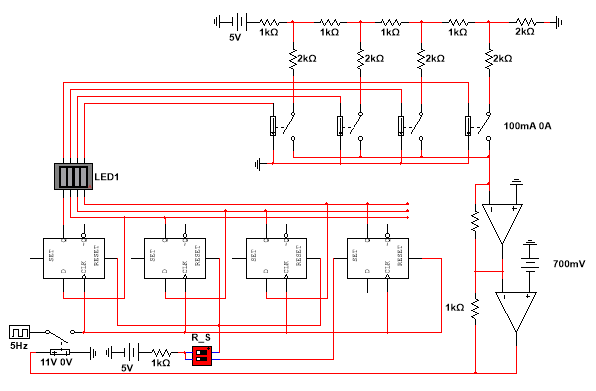
\includegraphics[scale=0.8]{images/image-6.png}
    \caption{АЦП последовательного приближения}
\end{figure*}